\documentclass{ani-final}
\usepackage[colorlinks=true,
     linkcolor=CadetBlue4,
     filecolor=CadetBlue4,
     citecolor=CadetBlue4,      
     urlcolor=CadetBlue4]{hyperref}
\usepackage{booktabs}
\usepackage{pdflscape}
\usepackage{multirow}

\usepackage{lipsum} % sampling purposes

\begin{document}


\frontmatter

\coverart{images/FARFETCH-logo.pdf}
\footerart{images/FUNDOS-3logos.pdf}
\reportnum{Technical Scientific Report}

\program{Final Technical Scientific Report}

\title{Incentive System for Research and Technological Development (R\&D) – Projects in Co-promotion\\International Partnerships}
\subtitle{}
\date{}

\reporttype{Final Report}

%\preparedfor{}

\maketitle

\tableofcontents

\listoffiguresandtables

\mainmatter

\chapter{Identification}

\begin{table}[!htp]
  \begin{tabular}{|l|p{.5\textwidth}|}
    \hline
    Project No.:                             & \\   \hline
    Project acronym:                         & \\   \hline
    Project title:                           & \\   \hline
    Project start date:                      & \\   \hline
    Project duration:                        & \\   \hline
    Reporting period:                        & \\   \hline
    Periodic report No.:                     & \\   \hline
    Project ``Web site'' or ``microsite'':   & \\   \hline
    Consortium composition:                  & \\   \hline
  \end{tabular}
\end{table}

\chapter{Project summary and general goals}
\lipsum[1-4]

\chapter{Gantt chart comparing the work planned in the application with the work carried out, duly commented}
\lipsum[1-2]

\begin{figure}[!htp]
  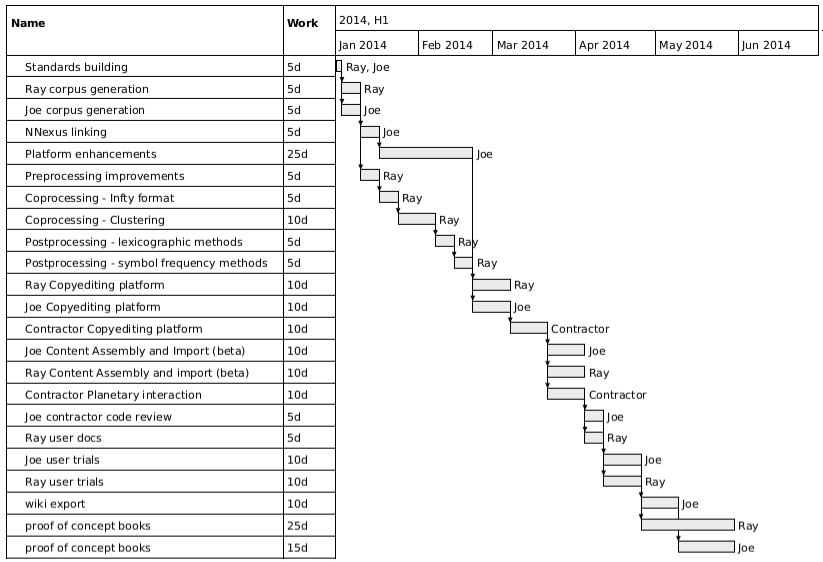
\includegraphics[width=1\textwidth]{images/gantt.png}
  \caption{A Gantt Chart (from \href{https://commons.wikimedia.org/wiki/File:Planetmathbooks_gantt.png}{wikimedia}).}
\end{figure}

\lipsum[3-4]


\chapter{Update and assess the degree of conformity with the project's innovative features}
\lipsum[1-4]

\newpage
\begin{landscape}
\begin{table}
  \centering
  \scriptsize
  \begin{tabular}{|p{0.2\textwidth}|p{0.1\textwidth}|p{0.2\textwidth}|p{0.2\textwidth}|p{0.2\textwidth}|p{0.2\textwidth}|}
    \hline
    Novel Features & Measure Unit & Market Assessment & Project Objectives & Relative Importance & Degree of Fulfillment \\ \hline
  \end{tabular}
  \caption{Innovative features and degree of fulfillment.}
\end{table}
\end{landscape}
\newpage


\chapter{Work and results accomplished since the project's beginning}
\lipsum[5-9]

  \section{Deliverables and milestones}
  \subsection{Deliverables}
  \lipsum[10-12]

  \newpage
  \begin{landscape}
    
    \begin{table}
      \centering
      \scriptsize
      \begin{tabular}{|p{0.1\textwidth}|p{0.1\textwidth}|p{0.2\textwidth}|p{0.1\textwidth}|p{0.1\textwidth}|p{0.1\textwidth}|p{0.1\textwidth}|p{0.2\textwidth}|p{0.3\textwidth}|}
        \hline
        Deliverable No. & Task No. & Deliverable Title & Deliverable Type & Scheduled Delivery Date of Annex B & Effective Delivery Date & If not delivered, why? & Disclosure Level & Comments \\ \hline
      \end{tabular}
      \caption{Deliverables.}
    \end{table}
  \end{landscape}
  
  \newpage
  \subsection{Milestones}
  \lipsum[10-12]

  \newpage
  \begin{landscape}
    \begin{table}
      \center
      \scriptsize
      \begin{tabular}{|p{0.1\textwidth}|p{0.1\textwidth}|p{0.2\textwidth}|p{0.4\textwidth}|p{0.1\textwidth}|p{0.1\textwidth}|p{0.1\textwidth}|p{0.1\textwidth}|p{0.1\textwidth}|}
        \hline
        Milestone No. & Task No. & Milestone Title & Verification Methods & Scheduled Delivery Date of Annex B & Effective Delivery Date Achieved & If not achieved, why? & Comments \\ \hline
      \end{tabular}
      \caption{Milestones.}
    \end{table}
  \end{landscape}
  \newpage



  \section{Promotion and dissemination of results}
  \lipsum[20-24]
  
  \begin{table}[!htp]
    \begin{tabular}{|p{0.75\textwidth}|p{0.25\textwidth}|}
      \hline
      \textbf{Typology of Action for Promotion and Dissemination of Results} & \textbf{Number of Actions} \\ \hline
      Conference organization                                          &  \\ \hline
      Workshop organization                                            &  \\ \hline
      Public demonstrations of prototypes, pilot lines                 &  \\ \hline
      Press-Release                                                    &  \\ \hline
      Non-scientific publications Scientific publications + Scientific publications co-authored with company(s) &  \\ \hline
      Participation in Trade Shows and Exhibitions                     &  \\ \hline
      Flyers                                                           &  \\ \hline
      Website                                                          &  \\ \hline
      Participation in Conferences                                     &  \\ \hline
      Participation in Workshops                                       &  \\ \hline
      Participation in Brokerage Events                                &  \\ \hline
      Others                                                           &  \\ \hline
    \end{tabular}
    \caption{Promotion and dissemination of results.}
  \end{table}


\chapter{Presentation of the results achieved by activity, justifying, if applicable, the deviations from what was foreseen in the application}
\lipsum[25-30]

\cite{sigfridsson}

\chapter{Financial implementation by promoter, presenting and justifying the deviations, by heading, in relation to that foreseen in the application}
\lipsum[30-32]

\chapter{Economic valuation of results}
\begin{table}[!htp]
  \centering
  \scriptsize
  
  \begin{tabular}{ll|p{0.1\textwidth}p{0.1\textwidth}p{0.1\textwidth}p{0.1\textwidth}}
    \hline\hline
    & & \textbf{It is not planned/ N/A} & \textbf{Needs new developments} & \textbf{In launch phase} & \textbf{In Commercial Exploration}  \\ \hline
    \multicolumn{2}{p{0.4\textwidth}|}{Degree of success in the commercialisation/exploration of the technology} & & & &\\ \hline
    \multirow{2}{*}{Target Market} & National Market & & & & \\ \cline{2-6}
                                   & External Market & & & & \\ \hline
    \hline
  \end{tabular}
  \caption{Economic value.} 
\end{table}

\section{Direct impact on the product/customer portfolio (post-project) of the company(ies)}

\textbf{FARFETCH}

\begin{table}[!htp]
  \centering
  \scriptsize
  
  \begin{tabular}{p{0.4\textwidth}|p{0.1\textwidth}p{0.1\textwidth}p{0.1\textwidth}p{0.1\textwidth}p{0.1\textwidth}p{0.1\textwidth}}
    \hline\hline
                         & \textbf{Current Customers} & \textbf{New Customers/Same Geographies} & \textbf{Same Customers/New Geographies} & \textbf{Spin-off Created by \emph{ESCT}} & \textbf{N/A}\\ \hline
    Creation of a broadcasting company & & & & &\\ \hline
    New area of Market                 & & & & & \\ \hline
    New product range / new process    & & & & & \\ \hline
    Improvement of existing product/service/process & & & & & \\ \hline
    \hline
  \end{tabular}
  \caption{Direct impact created by the project.} 
\end{table}

\chapter{Commercialization Strategies}
\begin{table}[!htp]
  \centering
  \scriptsize
  
  \begin{tabular}{c|p{0.3\textwidth}p{0.3\textwidth}p{0.3\textwidth}}
    \hline\hline
    \textbf{Year} & \textbf{Sales value + services resulting of the project} & \textbf{Percentage of the value of sales + services rendered resulting from the project in the total expected turnover of the company} & \textbf{Value of exports resulting from the project}\\ \hline
    n   & & & \\ \hline
    n+1 & & & \\ \hline
    \hline
  \end{tabular}
  \caption{Prospective Impact of the Strategy.} 
\end{table}

\chapter{Other Impacts}

\chapter{Appendix}

\nocite{*}
\bibliographystyle{unsrt}
\bibliography{biblatex-examples}

\end{document}
